\documentclass[11pt,landscape]{article}
\usepackage[a3paper]{geometry}
\usepackage{graphicx}
\usepackage{fancyhdr}
\usepackage{multirow}
\usepackage{multicol}
\usepackage{textcomp}
\usepackage{gensymb}
\usepackage{amsmath, amssymb}
\usepackage{float}
\usepackage{wrapfig}
\usepackage{hyperref}
\usepackage[parfill]{parskip}
\usepackage{glossaries}
\usepackage{amsmath}
\usepackage{mdframed}
\usepackage{caption}
\geometry{margin=2.5cm}

\graphicspath{{./images/}}

\pagestyle{fancy}
\setlength{\headheight}{24pt}
\fancyhead[L]{GDP Group}
\fancyhead[R]{Design of Smart Autonomous Golf caddy}
\fancyfoot[C]{\thepage}


\title{GDP Draft Report}
\author{GDP Group}



\begin{document}
\pagenumbering{arabic}
\maketitle
\newpage
\begin{multicols}{3}
\tableofcontents
\newpage
\section{Introduction}
The primary goal of this project is to construct a fully autonomous golf caddy.
There are caddies with varying ranges of autonomy available on the market
alread, from just having a motor so that no pushing from the golfer is required,
to being able to automatically following the golfer. There is currently no
product available that requires no operation from the golfer after the power up
phase. The currently available models that can follow the golfer would follow
them into a bunker, onto the green, or onto water if not prevented by a remote
control operated by the golfer.

Currently it is against golf association rules for any tools which indicate
which club should be used to be employed by golfers. Our sponsor James Siabati
indicates that this may change in the near future, so including this ability in
our autonomous caddy is a good decision.
\section{Project Aim and Objectives}
\section{Design Criteria}
\section{Mechanical Design}


\section{Software}
\label{software}
In this section all software required for the operating cycle of the AGC is
discussed. The AGC main computer is a Raspberry Pi 4 running a 64-bit Debian port,
the same is true for the Raspberry Pi used in the tracking pod. The GPS
navigation system requires high precision decimal storage to operate properly.
Data type \verb|float32| can store 23 significant bits, compared to data type
\verb|float64| which can store 52 significant
bits\cite{floating_point_goldberg}. 
The calulcations shown below in Fig. (\ref{fig:float_calcs}) show the
physical significance of which datatype is chosen.
\begin{figure}[H]
    \begin{mdframed}
        Only $180^{\circ}$ need to be accounted for because sign bit is separate, so to
        represent $180^{\circ}$ the bits required is:
        \begin{center}
            \begin{equation*}
                \log_2{180} \approx 7.49185 bits
            \end{equation*}
        \end{center}
        This leaves the $n - 7.49185$ significant bits left for sub degree
        representation, the physical precision in meters we can then derive from each
        data type of a longitude value at the equator can be calculated as shown in
        Eqs. () respectively.\newline
        \begin{center}
            \begin{minipage}{0.45\textwidth}
                \begin{mdframed}
                    For \verb|float32| $n=23$:
                    \begin{center}
                        \begin{equation*}
                            \frac{\frac{R_e \cdot \pi}{180}}{2^{\left(52 - \log_2{180}\right)}} \approx 2.386m
                            \label{eq}
                        \end{equation*}
                    \end{center}
                \end{mdframed}
                \end{minipage}
                \begin{minipage}{0.45\textwidth}
                    \begin{mdframed}
                For \verb|float64| $n=52$:
                \begin{center}
                    \begin{equation*}
                        \frac{\frac{R_e \cdot \pi}{180}}{2^{\left(52 - \log_2{180}\right)}} \approx 4.44nm
                    \end{equation*}
                \end{center}
            \end{mdframed}
            \end{minipage}
        \end{center}
        \center The radius of Earth. $R_e$, value used was $6371000m$. 
    \end{mdframed} 
    \captionof{figure}{Calculations showing physics precision of single vs double
    precision floats}
    \label{fig:float_calcs}
\end{figure}
The $180^{\circ}$ is normalised to a power of two so we are able to use the non
integer value of bits in the calculation for physical precision, were we to not
perform this normalisation then $7.4918\rightarrow8$ full bits are required to
represent the degrees and the final
precision is slightly less for each datatype. To ensure this calculated
precision is representative of our system all GPS coordinates are normalised to
a power of two. We can see from the calculations that a significantly higher
precision is achieved using double precision floating point data type to store
GPS values. The precision yielded by the double precision floating point is
unnecessary, however the precision of the single precision floating point is too
low as our GPS module is capable of providing more accurate GPS measurements as
discussed in section \ref{electronics}. Therefore double precision floating
point datatypes will be used to store GPS data, which requires us to use a
64-bit compatible operating system which is why the 64-bit Debian port was
chosen. The higher precision achieved comes at the cost of slightly higher
compte time for calculations, however as most of the algorithms onboard operate
only on small amounts of data, this effect is unnoticable when operating the
AGC.

\subsection{Control Software}
\label{control_software}
This section discusses the software used to make the AGC follow the golfer.
All of the control software apart from the elctronics specific code, such as
motor controller communication, was written first using the OpenGL simulator
that was built throughout the year. Building and using a simulator allowed us to 
write and test all the control software / algorithms that would be required to make 
the AGC follow the golfer as intended while avoiding hazard regions.

All of the control software tested in the simulator was written in C as this was
easiest to use with OpenGL, however we decided to change to PyQt5 for designing
the onboard GUI. As the ACG software was now to be written in Python the control
algorithms were re-written in Python, however upon testing it was found that
their performance was significantly slower than the C implementations. This is
most likely a large number of array passing and manipulations are required,
which is significantly slower in Python where function arguments are passed as
object reference instead of pointers in C. Therefore the original C control
algorithms were compiled as a dynamic link library (DLL) and the Python ``C
Types'' library was used to load the DLL and create Python wrappers for the control
algorithms. This significantly improved the performance as all of the resource
intensive calculations were now performed with a compiled C program.

The main control loop that determines the AGC's behaviour is shown below in
Fig. (\ref{fig:control_loop}).
\begin{figure}[H]
\begin{mdframed}
    \begin{center}
        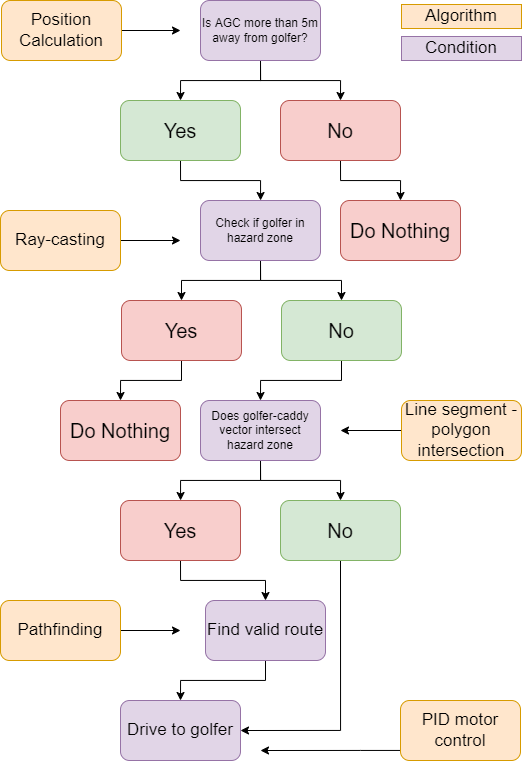
\includegraphics[width=0.9\textwidth]{control_loop.png}
    \end{center}
\end{mdframed}
\captionof{figure}{Main AGC control loop}
\label{fig:control_loop}
\end{figure}
\subsubsection{Map Processing}
As discussed in the introduction to section \ref{software}, all GPS
coordinates are normalised to a power of two. We also ``pad'' the hazard zone
coordinates, before normalisation, by a safety factor of two meters, preventing innacurate GPS
readings or hazard zone coordinates resulting in the AGC entering a hazard zone.
We ``pad'' the hazard zones by calculating the coordinates of centroid of the
polygon, then extending the vector from the centroid to each perimeter point by
two meters. The centroid of a polygon can be calculated from the coordinates of
it's perimeter points as shown in Eqs. (\ref{eq:cx} and \ref{eq:cy}).
\begin{center}
    \begin{equation*}
        A=\frac{1}{2}\sum_{i=0}^{n-1}\left( x_i y_{i+1} - x_{i+1} y_i\right)
    \end{equation*}
\end{center}
\begin{center}
    \begin{equation}
        C_x=\frac{1}{6A}\sum_{i=0}^{n-1} (x_i + x_{i+1}) (x_i y_{i+1} - x_{i+1} y_i)
        \label{eq:cx}
    \end{equation}
\end{center}
\begin{center}
    \begin{equation}
        C_y=\frac{1}{6A}\sum_{i=0}^{n-1} (y_i + y_{i+1}) (x_i y_{i+1} - x_{i+1} y_i)
        \label{eq:cy}
    \end{equation}
\end{center}
\subsubsection{Ray Casting}
The ray casting algorithm is used to determine whether a point falls within a
polygon. The algorithm can only accept polygons with straight edges; our polygons are
represented by a series of GPS points along their perimeter, and so our polygons
are defined by a series of small straight edges. The concept of this algorithm
is that given a point you wish to test, if you cast a ray from the point in one
direction to infinity, the number of intersections the ray has with the polygon
in question indicates whether the point falls in the polygon or not. If an even
number of intersections are found, then the point lies outside the polygon, and
if an odd number of intersections are found the point lies within the polygon.
A visual of this concept can be seen below in Fig. (\ref{fig:raycasting}).
\begin{figure}[H]
    \begin{mdframed}
        \begin{center}
            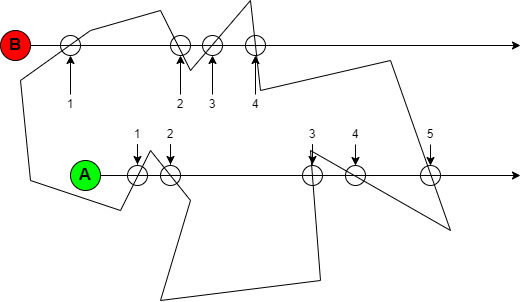
\includegraphics[width=0.95\textwidth]{raycasting.png}
        \end{center}
    \end{mdframed}
    \captionof{figure}{Raycasting Example}
    \label{fig:raycasting}
\end{figure}

The figure shows two points which are to be tested to determine if they lie
within the polygon. Casting the ray to the right, towards $x\rightarrow\inf$ in
our implementation, we can count the intersections each ray has with the
polygon. Point A has five intersections and so lies outside the polygon, point B
has four intersections and lies within the polygon. 

There are additional considerations in our implementation to accout for the ray
intersecting a vertex or for the ray being collinear with a polygon edge. If a
vertex is intersected then two intersections are counted, one for each edge
forming the vertex, and the result is not affected. If the ray is collinear
with a polygon edge then only a single intersection is counted, but the ray will
undoubtedly also intersect at least one of the vertices on the collinear edge
which will be appropriately accounted for.
The algorithm has been tested and does not fail in either of these cases.

\subsubsection{Segment Polygon Intersection}
Before the AGC starts moving towards any target destination, it first checks
that it's intended translation vector joining it's location to the target
location does not pass through
any hazard zones. It does this by checking that it's intended translation vector
doesn't intersect any edges of polygons. The diagram shown below in Fig.
(\ref{fig:segment_intersection}) depicts two finite length line segments
intersecting.
\begin{figure}[H]
    \begin{mdframed}
        \begin{center}
            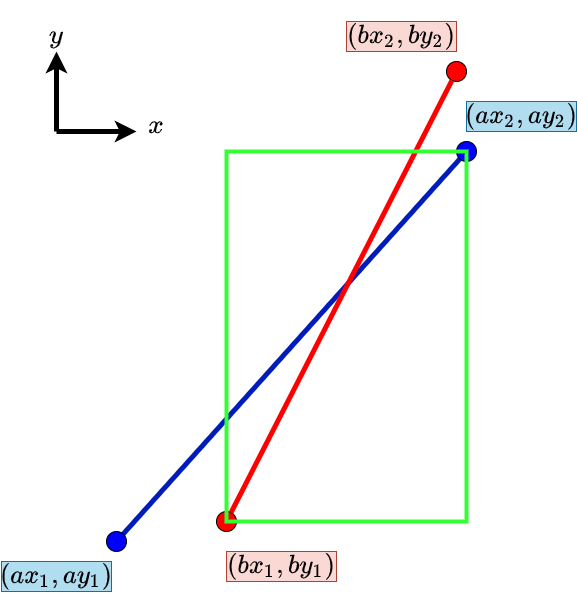
\includegraphics[width=0.95\textwidth]{segment_intersection.png}
        \end{center}
    \end{mdframed}
    \captionof{figure}{Line Segment Intersection Diagram}
    \label{fig:segment_intersection}
\end{figure}
 
The edges of polygons are defined only by the positions of two vertices, as is
the AGC intended translation vector. To calculate where the intersection point
of these two line segments are a mathematical equation for a line must be
constructed for each segment as shown in Eqs. (\ref{eq:line_a} and
\ref{eq:line_b}) respectively, then these equations can be solved simultaneously
to determine the location of the intersection as shown in Fig.
(\ref{fig:segment_calculations}).

After the intersection point is calculated we ensure that the intersection point
falls within the smallest rectangle bounded by one point from the first and
second coordinates of either segment. We do this because the equation for a line is infinite, and
any lines with non equal gradient will intersect, but we are only interested if
the intersection occurs between points the AGC intends to travel. The bounding
rectangle is demonstrated by the green rectangle in Fig. (\ref{fig:segment_intersection}).

\begin{figure}[H]
    \begin{mdframed}
        \begin{center}
            \begin{equation}
                ay_1-y = \frac{ay_2 - ay_1}{ax_2 - ax_1} \times (x - ax_1)
                \label{eq:line_a}
            \end{equation}
            \begin{equation}
                by_1-y = \frac{by_2 - by_1}{bx_2 - bx_1} \times (x - bx_1)
                \label{eq:line_b}
            \end{equation}
        \end{center}
    In our implementation, before this system is solved, we check
    if the lines have equal gradient, and if they are collinear or not. If they
    have equal graident, defined by:
    \begin{center}
        \begin{equation*}
            \frac{ay_2 - ay_1}{ax_2 - ax_1} = \frac{by_2 - by_1}{bx_2 - bx_1}
        \end{equation*}
    \end{center}
    Then we check if they are collinear, defined by:
    \begin{center}
        \begin{equation*}
            (x - ax_1) = (x - bx_1)
        \end{equation*}
    \end{center}
    If they are collinear then they intersect, if the have equal gradient but
    are not collinear then they do not intersect. If one or both of the lines
    are vertical, $(y_1 = y_2)$ then the system is not solved as below but
    trivially using the $x$ position of the line.\vspace{0.5cm}
    \newline
    For simplification:
    \begin{center}
        \begin{equation*}
            m_a = \frac{ay_2 - ay_1}{ax_2 - ax_1} \hspace{1cm} m_b = \frac{by_2 - by_1}{bx_2 - bx_1}
        \end{equation*}
    \end{center}
    Now we solve the system defined by Eqs. (\ref{eq:line_a} and
    \ref{eq:line_b}) to determine the point of intersection resulting in the $x$
    coordinate given by Eq. (\ref{eq:x}) and $y$ coordinate given by Eq. (\ref{eq:y}).
    \begin{center}
        \begin{equation}
            x = \frac{ax_{1} m_{a} - ay_{1} - bx_{1} m_{b} + by_{1}}{m_{a} - m_{b}}
            \label{eq:x}
        \end{equation}
        \begin{equation}
            y = \frac{ax_{1} m_{a} m_{b} - ay_{1} m_{b} - bx_{1} m_{a} m_{b} + by_{1} m_{a}}{m_{a} - m_{b}}
            \label{eq:y}
        \end{equation}
    \end{center}
    \end{mdframed}
    \captionof{figure}{Calculation of Line Segment Intersection Point}
    \label{fig:segment_calculations}
\end{figure}

\subsubsection{Pathfinding}
The pathfinding algorithm is only used if the control loop shown in Fig.
(\ref{fig:control_loop}) determines that the AGC should move to the golfer but
the a direct route is not possible due to the presence of a hazard zone between
them. Initially the A* pathfinding algorithm was researched as it is a well known algorithm
with which we could choose some heuristic function to minimise, in our case that
heuristic function would likely be the shortest distance to reach the golfer.
 A* is generally used
for pathfinding on a discrete graph, we do not have a discrete graph
available and so would have to construct one for each golf course or a local graph
surrounding the hazard we wish to avoid. This adds unnecessary complexity in
terms of implementation and computation to our system which we wish to avoid.
Additionally, A* has time complexity of $O(b^d)$ if $d$ is the shortest path length
and b is the branching factor, and the algorithm has high memory requirements as all generated
nodes are kept in memory \cite{astar_2009}. It
was decided we would not use A* algorithm. The next consideration was to simply
``pad'' the perimeter of the hazard polygon and follow it all the way around
until the AGC reaches the golfer. This concept is shown in
the diagram below in Fig. (\ref{fig:padding}) where the red line denotes
the path that would be taken by the AGC to avoid a hazard zone. Clearly this is
an inefficient path the AGC will unnecessarily follow the contour of the
polygon. Additionally, this method increases the risk that the AGC enters the
hazard zone if our GPS system is not performing well, or if our GPS mapping of
hazard zones is erronous.  


\begin{figure}[H]
    \begin{mdframed}
        \begin{center}
            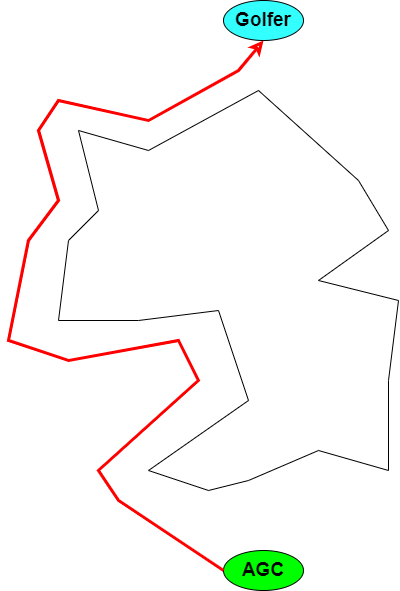
\includegraphics[width=0.95\textwidth]{padding.png}
        \end{center}
    \end{mdframed}
    \captionof{figure}{Path derived by ``padding'' polygon}
    \label{fig:padding}
\end{figure}

A custom pathfinding algorithm was designed and implemented. The path it finds
is not the optimal solution, but it computes quickly and the path derived is
more efficient than using the ``padding'' method. Fig.
(\ref{fig:pathfinding_flow}) shows the main steps performed by the algorithm to
determine where the AGC should go.

\begin{figure}[H]
    \begin{mdframed}
        \begin{center}
            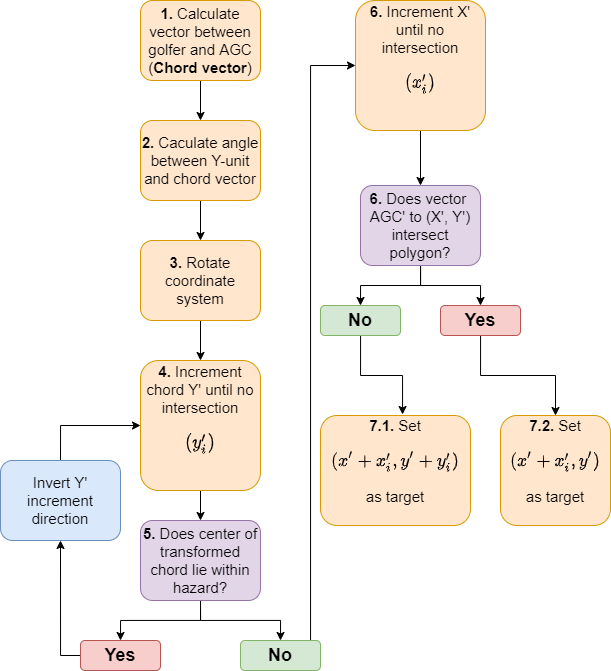
\includegraphics[width=0.95\textwidth]{pathfinding_flow.png}
        \end{center}
    \end{mdframed}
    \captionof{figure}{Pathfinding algorithm main steps}
    \label{fig:pathfinding_flow}
\end{figure}

First the chord vector, $\overrightarrow{\mathbf{C}}$, is calculated, along with
the angle, $\theta$, between $\overrightarrow{\mathbf{C}}$ and the Y-unit vector,
$\hat{\mathbf{y}}$, using Eq. ().  The relevant polygon, golfer position, and AGC
position are rotated about the z-axis with the center of rotation as the
origin by $\theta$ using Eq. () where $\overrightarrow{p}$ is a
three dimensional point and $\overrightarrow{p^\prime}$ is the rotated point. 
The polygon is rotated by applying Eq. () to each
vertex. The purpose of the rotation was to aid the design process of the
algorithm and make the code more readable, removing the necesscity for vector
manipulations throuhout the algorithm instead using only simple arithmetic operations.
This results in $\overrightarrow{\mathbf{C}^\prime}$ having constant $y$. The
value of $y^\prime$ is increment in one meter steps until no intersection
between the translated chord vector, $\overrightarrow{\mathbf{C}^\prime_t}$, and
the rotated polygon, $\mathbf{P}^\prime$. If any point of
$\overrightarrow{\mathbf{C}^\prime_t}$ lies within the polygon the increment
direction is reversed and incremented until there is no intersection and no
points of $\overrightarrow{\mathbf{C}^\prime_t}$ lie within the polygon. This
increment process is repeated in the $x^\prime$ direction for the vector joining
the rotated AGC position,
$\left(x^\prime_{AGC}, y^\prime_{AGC}\right)$, to $\left(x^\prime_{AGC},
y^\prime_{AGC} + y^\prime_i\right)$. Once the incrementation process if finished
such that no intersections are found, the vector joining $\left(x^\prime_{AGC},
y^\prime_{AGC}\right)$ to $\left(x^\prime_{AGC}+x^\prime_i,
y^\prime_{AGC} + y^\prime_i\right)$ is checked for intersections. If none are
found then $\left(x^\prime_{AGC}+x^\prime_i,
y^\prime_{AGC} + y^\prime_i\right)$ is rotated back to the original coordinate
system and set as the position target for the AGC. If an intersection is found
then $\left(x^\prime_{AGC}+x^\prime_i, y^\prime_{AGC}\right)$ is rotated back to
the original coordinate system and set as the AGC position target. This process
repeats until the golfer is reached. Incrementing in the $y^\prime$ direction
is equivelant to incrementing perpendicular to
$\overrightarrow{\mathbf{C}}$ in
the original coordinate system, and incrementing it by $x^\prime$ is equivelant
to incrementing in the direction of $\overrightarrow{\mathbf{C}}$.
\subsubsection{Pathfinding Diagram}
Fig. (\ref{fig:pathfinding_visual}) shows a visual of how the pathfinding algorithm will determine intermediary
positions for the AGC to move it towards the golfer. For the generation of this
figure the pathfinding algorithm was only called again after the target position
is reached, resulting in the very wide path that can be seen in the final path
diagram. On the AGC the pathfinding algorithm is called every time new GPS data
is available, approximately every second, resulting in a smoother and closer
path being found.
\end{multicols}
\newpage
\begin{figure}[H]
    \begin{mdframed}
        \begin{center}
            \begin{minipage}{0.3\textwidth}
                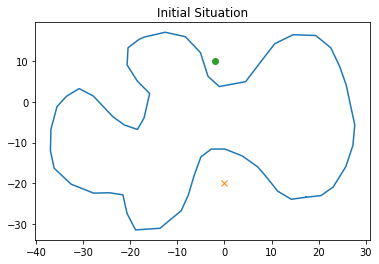
\includegraphics[width=0.95\textwidth]{initial.png}
            \end{minipage}
            \begin{minipage}{0.3\textwidth}
                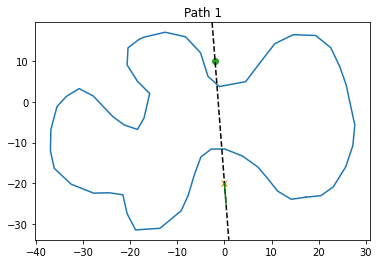
\includegraphics[width=0.95\textwidth]{p1.png}
            \end{minipage}
            \begin{minipage}{0.3\textwidth}
                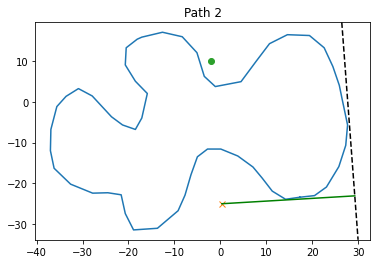
\includegraphics[width=0.95\textwidth]{p2.png}
            \end{minipage}
        \end{center}
        \begin{center}
            \begin{minipage}{0.3\textwidth}
                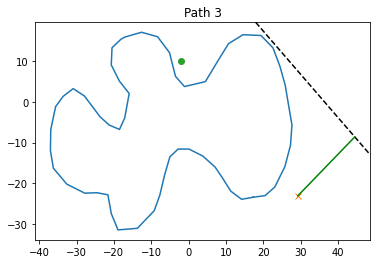
\includegraphics[width=0.95\textwidth]{p3.png}
            \end{minipage}
            \begin{minipage}{0.3\textwidth}
                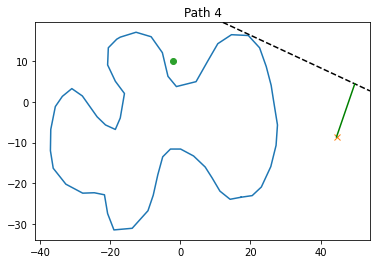
\includegraphics[width=0.95\textwidth]{p4.png}
            \end{minipage}
            \begin{minipage}{0.3\textwidth}
                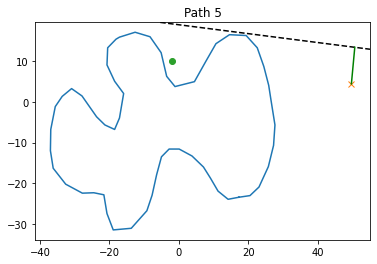
\includegraphics[width=0.95\textwidth]{p5.png}
            \end{minipage}
        \end{center}
        \begin{center}
            \begin{minipage}{0.3\textwidth}
                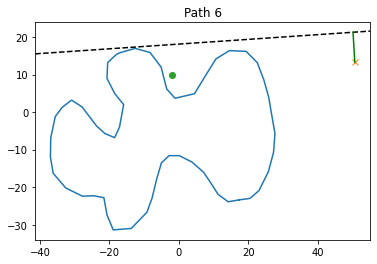
\includegraphics[width=0.95\textwidth]{p6.png}
            \end{minipage}
            \begin{minipage}{0.3\textwidth}
                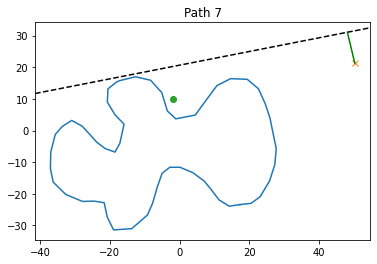
\includegraphics[width=0.95\textwidth]{p7.png}
            \end{minipage}
            \begin{minipage}{0.3\textwidth}
                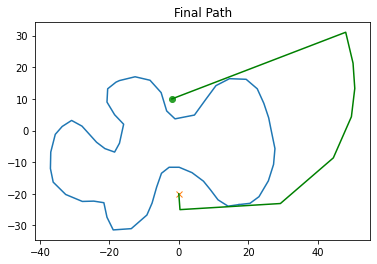
\includegraphics[width=0.95\textwidth]{final.png}
            \end{minipage}
        \end{center}
    \end{mdframed}
    \captionof{figure}{Visualisation of path determined by pathfinding algorithm}
    \label{fig:pathfinding_visual}
\end{figure}
\newpage

\begin{multicols}{3}

\subsection{Communications}
The EMG30 motors we are using are controlled by the MD25 motor controller board
via and $I^2C$ interface. The communication interface for this was written in C
and is capable of handling multiple $I^2C$ devices. Currently the only device we
have on the communications network is the MD25. The GPS in the golfer's pod communicates to the main Raspberry Pi via Bluetooth,
which is written in Python using the PyBluez library. The GPSs communicate with
the Raspberry Pis via serial commuication implemented using the Pyserial
library.

\subsection{GUI}
\subsubsection{Course Map}
The course map was implemented on the GUI using the map system that was used on
the simulator. We attempted to embed a map web app called folium which looks
better than the map developed for the simulator, however, it doesn't allow us to
retreive coordinates for a point clicked on the map in real latitude / longitude
coordinates or in screen coordinates. This shortfall makes it impossible to give
the golfer the ability to click a point on the map and see how far away it is
from the AGC, using the simulator map allows us to add that feature.



\section{Electronics}
\label{electronics}
\subsection{Motors}
The motors we decided to use for our prototype version are the EMG30 motors
because we already have them and this will save cost. However, they are
underpowered as they will take too long to accelerate the AGC to full speed, and
won't work at on anything more than a slight incline; for a final version the
EMG49 motors should be used. 
We chose these motors
by
considering the top speed we wish the AGC to able to go, and how fast we want it
to accelerate to that speed on a $10^\circ$ incline. The calculations shown below in
Fig. (\ref{fig:motor_calcs}) show how we calculated the necessary toruqe and rpm we require from our
motors.

\begin{figure}[H]
    \begin{mdframed}
        The top speed we chose for the AGC was 5.0 kilometers per hour,
        equivalent to average walking speed. 
        The wheel radius, $W_r$ of the AGC wheels is 0.115 meters. We can
        calculate RPM using Eq. (\ref{eq:rpm}):
        \begin{center}
            \begin{equation}
                rpm = \frac{7.5 * \frac{1000}{3600}}{2\pi W_r} \cdot 60 \approx 115rpm
                \label{eq:rpm}
            \end{equation}
        \end{center}
        The AGC should be able
        to accelerate to this speed, $V$, within $t=5$ seconds on a $10^\circ$ incline.
        For predicted final mass, $M = 15kg$, 
        the accelerating force, $F$, required can be calculated with Eq. (\ref{eq:accel}):
        \begin{center}
            \begin{equation}
                F = \frac{V}{t} + M g_0 \sin(10^\circ)\approx 29 N
                \label{eq:accel}
            \end{equation}
        \end{center}
        Finally the torque required from each motor can bel calulated using Eq.
        (\ref{eq:torque}):
        \begin{center}
            \begin{equation}
                T = W_r * F \approx 1.7 Nm
                \label{eq:torque} 
            \end{equation}
        \end{center}
    \end{mdframed}
    \captionof{figure}{Motor requirement calculations}
    \label{fig:motor_calcs}
\end{figure}

According to their datasheet the EMG49 motors can provided a loaded rpm of 122
and a torque of 1.56, close to our requirements set out above. As the torque is
slightly lower than calulated, the AGC will accelerate slightly to top speed on
a $10^\circ$ incline in slightly over five seconds.

\newpage
\nocite{*}
\bibliographystyle{ieeetr}
\bibliography{./ref}
\end{multicols}



\end{document}